\documentclass[]{final_report}
\usepackage{graphicx}
\usepackage{hyperref}
\usepackage{listings}


%%%%%%%%%%%%%%%%%%%%%%
%%% Input project details
\def\studentname{Ciaran Palmer}
\def\projecttitle{SensorML on SenseTile}
\def\supervisorname{Your Supervisor Name}
\def\moderatorname{Your Moderator Name}


\begin{document}

\maketitle
\tableofcontents\pdfbookmark[0]{Table of Contents}{toc}\newpage

%%%%%%%%%%%%%%%%%%%%%%
%%% Your Abstract here

\begin{abstract}
SenseTileSensor Board

SensorML description.

WebServer to access sensor observations

SensorML Bon Mapping with a tool and method to develop sensorML descriptions

\end{abstract}




\newpage


%%%%%%%%%%%%%%%%%%%%%%
%%% Acknowledgments

\chapter*{Acknowledgments}

Vieri del Bianco , Dragan Stosic and Joseph R. Kiniry.

%%%%%%%%%%%%%%%%%%%%%%
%%% Introduction

\chapter{Introduction}

problems.

Sensor Networks are increasingly deployed to provide sensing information for a myriad of applications. These Sensor Networks are developed by communities working in different domains and contain many different sensor types. The heterogeneity of these systems means that interoperability is difficult and expensive. Reliably processing sensor observations from these heterogeneous systems is also issue. Need to have a sensor description, data description, observation, retrieval and information on accuracy etc for reliable processing. Standards are being developed to address these problems. Use internet.

Sensor Model Language (SensorML)\cite{SMLref} is one proposed standard for sensor description and processing of sensor observations. SensorML specifies models and XML Schema for describing sensors, the process of sensor measurement and the post processing of sensor observations. 

The Sensor Observation Service (SOS)\cite{SOSref}  specification is a proposed standard for retrieving information about sensor and retrieving sensor observations. 

The SensorML and SOS specifications are developed by the Open Geospatial Consortium (OGC) as part of the Sensor Web Enablement (SWE) initiative \footnote{http://www.opengeospatial.org/projects/groups/sensorweb}. The members of the OGC have the goal of improving interoperability of sensor systems by developing open standards such as SensorML. This thesis investigates the use of these standards in developing sensor systems.

Currently there is no formal definition of sensors or sensor data processing. There are now formal verification based software development processes [kiniry] with the goal of developing very robust systems. Having formal sensor descriptions allows sensor system development with such a verification based process.

The thesis uses a real sensor system called SenseTile as a case study. SenseTile is a sensor and processing package that can contain motion sensors, RFID sensors, temperature sensors, audio sensors, pressure sensors, light level sensors video sensors among others. It is used as a replacement for standard ceiling tiles to provide smart building services as part of a Web Sensor Network.

This thesis describes SenseTile with SensorML. Based on this model a SenseTile Web Service prototype is developed to allow the retrieval of the sensor SensorML descriptions and sensor observations to be retrieved. The Web Service will be based on the SOS specification. An assessment of SensorML and SOS is provided based on this work.

To formalize sensor description and process BON\cite{BONref} is a notation and a method for Object Oriented systems analysis and design. A BON to SensorML mapping is provided. The proposed approach would allow sensor processing to defined formally in BON and then refined to JML/Java.


\chapter{ Background Research}

\section{Sensor Web Enablement}
SensorML is developed as part of the Open Geospatial Consortium (OGC) Sensor Web Enablement (SWE) initiative \footnote{http://www.opengeospatial.org/projects/groups/sensorweb}. This initiative is establishing interfaces and protocols to enable a standardized Sensor Web. It is hoped that this allows for easier integration and development of sensor applications across sensor networks. The OGC SWE provides a framework of open standards for use with Web-connected sensors and sensor systems. There are seven main specifications currently:

\begin{itemize}
\item  SensorModel Language(SensorML) - models and schema for sensor systems and processes surrounding measurements
\item  Sensor Observation Service (SOS) - standard web interface for accessing observations
\item  Observations \& Measurements (O\&M) - models and schema for packaging observation values
\item  Transducer Markup Language (TML) - models and schema for multiplexed data from sensor systems
\item  Sensor Planning Service (SPS) - standard web interface for tasking sensor systems and model and requesting acquisitions
\item   Sensor Alert Service (SAS) - standard web interface for publishing and subscribing to sensor alerts
\item   Web Notification Service (WNS) - standard web interface for asynchronous notification
\end{itemize}

SWE services based on the aboved specifications allow the discovery of sensors, access to the sensor data, as well as subscription to alerts, and tasking of sensors to control observations. For a good overview of SWE and it's use in Sensor Web Network see \cite{SWEArchref}.  SensorML, SOS and O\&M specifications are the focus of this thesis and are described in more detail in the following sections.


\section{Sensor Modeling Language}\label{SMLsection}
Sensor Modeling Language (SensorML) is primarily used to describe sensor systems and the processing of observations from sensor systems. The SensorML specification\cite{SMLref} provides a functional model of sensors and an XML encoding to describe sensors and their observations. Some of the main uses of SensorML described in the specification are:
\begin{itemize}
\item support sensor and sensor observation discovery.
\item support processing of the sensor observations.
\item support geolocation information about sensors.
\item provide accuracy information of sensors measurements.
\item provide an explicit description of the process by which an observation was obtained.
\item provide an executable process chain for deriving new data products on demand.
\end{itemize}

In SensorML sensors are modeled as processes that convert real phenomena to data. Processes take inputs, process them and result in one or several outputs. For example, a process can take a measurement generated by a thermistor which might be a resistance value and transform it to a celcius value. Processes can also be connected together in process chains to allow the sensor data to be processed by several processes sequentially. These processes and process chains are modeled in SensorML as shown in the  below SensorML Conceptual Model \ref{fig:SMLConceptualModel}.

\begin{figure}[h]
\framebox{\scalebox{0.65}{\includegraphics{SMLConceptualModel.png}}}
\caption{SensorML Conceptual Model}\label{fig:SMLConceptualModel}
\end{figure}

Processes in SensorML derive from AbstractProcess with it's inputs, output, parameters and metaDataGroup properties. The inputs and outputs represent data connections to other processes. Parameters represent inputs other than sensor measurements or outputs of other processes. They are used to configure the process or provide other inputs that are not sensor measurements. For example a parameter might be the latency time of a measurement needed for a calculation. Finally each process provides sensor metadata as modeled by the MetaDataGroup.

SensorML divides processes into two types, physical and non-physical. The non-physical process is one where  location, position etc. is not relevant to the process. Physical processes provide physical information, such as location, which can be used in processing if required. The ProcessModel is a non-physical process while the Component is a physical process and contains extra properties for defining the needed spatial or temporal information. Both process types contain the processMethod property which points to the methodology for transforming inputs to outputs.

There is a similar division of the process chains into the non-physical ProcessChain and physical System. Both process chains can contain a mixture of ProcessModel and Component process if desired. Process chains have inputs and outputs which define the beginning and end of the processing chain. They are points of connection to other processes and process chains if needed. The connection property contained in the ProcessChain and System is a list of Link type. The Link type contains source and destination properties that reference inputs and outputs of the processes in the process chain thus connecting the processes. 

The SensorML specification currently contains the Sensor Web Enablement (SWE) Common specification. This specification defines basic types and data encodings used by the SWE specifications. It describes both primitive data types as well as aggregate types such as arrays and records. There are a large number of types defined in this specification, too many to show here. Below is a Conceptual Model of some of the simple data types.

\begin{figure}[h]
\framebox{\scalebox{0.65}{\includegraphics{SWESimpleConceptualModel.png}}}
\caption{SWE Common Simple Data Types.}\label{fig:SWESimpleConceptualModel}
\end{figure}

The data types in \ref{fig:SWESimpleConceptualModel} are scalar primitive values. They are the basis for the inputs, outputs and parameters in SensorML processes. Quantity models a floating point number. Count models a counting value or integer.  Boolean models a property that can be true or false. These types contain a number of properties that further define the type. The uom property provides a unit of measurement that indicate how the value should be interpreted.  A constraint property allows a value range or a enumerated list of values to be defined for the type. The quality property allows for a measure of its quality, for example the confidence level of a value being correct expressed as a percentage. Aggregation of these primitive data types is also provided by several types including DataRecord and DataArray.

SensorML uses XML Linking Language (XLink) \footnote{http://www.w3.org/TR/xlink} to support hypertext referencing in SensorML XML documents using URNs and URIs. This allows SensorML models to be distributed over several documents. XLink attributes are also used to reference on-line unit definitions used to define a sensor measurement.

The XML encoding of the SensorML model is not described here. The OGC SWE specification uses XML Schema to define the allowable SensorML XML structure.It is noted here that sml is the XML namespace for SensorML and swe is the XML namespace for SWE Common. In the later SenseTile SensorML model section examples of the XML encoding are used to describe the SenseTile Model. 

\section{Sensor Observation Service}
SensorML is envisioned to be used in conjunction with a Sensor Observation Service as described in the SWE Architecture \cite{SOSref}. The SOS defines a web service interface for the discovery of sensors systems and the retrieval of observations from sensor systems. It organizes related sensor observations into a collection called an observation offering.   

The SOS specification uses four main entities to describe the SOS's operation. The entities are Data Consumers, Data Producers, OGC Catalogs and the SOS itself. Data Consumers are clients of the SOS that request sensor observations and sensor metadata. Data Providers are entities have to access to the sensor and have enough processing power to generate an XML encoding of the sensor's observations. These observations are sent over a network to the SOS. The OGC Catalog is used to find SOS instances. SOS instances act as access points to a Sensor Web Network and provide the Web Service for retrieval of sensor observations. The figure \ref{fig:SOSoperationContext} below shows the entities described in the SOS in an operation context.
\begin{figure}[h]
\framebox{\scalebox{0.65}{\includegraphics{SOSoperationContext.png}}}
\caption{SOS Operational Context}\label{fig:SOSoperationContext}
\end{figure}

The diagram above shows the core and transactional operations provided by an SOS. The core operations are GetCapabilities, DescribeSensor and GetObservations. These are mandatory operations used by Data Consumers to request sensor information.  The core operations perform the following function:
 \begin{itemize}
\item GetCapabilities  -   operation to retrieve SOS observation offering information.
\item DescribeSensor - operation to retrieve detailed information about the sensors.
\item GetObservation -   operation to obtain sensor observations.
\end{itemize}

The transactional operations are RegisterSensor and InsertObservation used by the Data Producer to provided sensor information and observations. The transactional operations supported are described in the following:
 \begin{itemize}
\item RegisterSensor - operation to register the Data Provider with the SOS.
\item InsertObservation - operation to update SOS with a sensor observation.
\end{itemize}

These operations are encoded in XML and are intended to be carried http  operations. The sensor observations contained in  GetObservation and InsertObservation operations are encoded according to the OGC O\&M Observations \cite{OMref}. Sensor systems metadata contained in DescribeSensor and RegisterSensor is defined in SensorML or TML.

The SOS Operation Context diargam also shows a discovery process involving the  Data Consumer and a OGC Catalog Service (CS-W) catalog. The Data Consumer uses a CS-W catalog to find SOS instances. The GetCapabilites are then used toward each of the SOS instances returned to find sensor systems that are of interest to the Data Consumer. The CS-W catalog is covered in a separate specification \cite{OGCcatref}. This not covered in any real detail in the SOS specification. The OGC Catalog Service is not explored in this thesis.

There are also six other operations the SOS refers to as enhanced operations. They are GetResult,
GetFeatureOfInterest, GetFeatureOfInterestTime, DescribeFeatureOfInterest,
DescribeObservationType, and DescribeResultModel. These operations are not covered in this thesis.

The SenseTile Web Service developed in this thesis is based on the concepts described in the Sensor Observation Service (SOS) specification. The SOS Data Consumer and SOS Data Provider entities will referred to a DataConsumer and DataProvider respectively in this thesis when describing the SenseTile Web Service.


\section{SenseTile}
A case study of the use of SensorML in sensor networks is based on the SenseTile System. SenseTile is a general purpose sensor system developed at UCD CASL \footnote{http://kind.ucd.ie/
products/opensource/SenseTile}. The SenseTile System is used to investigate issues arising with large scale sensor networking. SenseTile is made up of a sensor platform, a datastore, and a compute farm. The below figure shows a outline of this system. 
\begin{figure}[h]
\framebox{\scalebox{0.65}{\includegraphics{SenseTileDescription.png}}}
\caption{SenseTile System}\label{fig:SenseTileDescription}
\end{figure}
 The sensor platform is called the SenseTile Unit and is composed of one or more SenseTile Sensor Boards paired with a SenseTile Processor Unit. The Processor could be a PDA or small PC or any processing device that has a USB connection.  The Sensor Board has a USB connection used for communication with the Processor Unit. There are over a dozen sensors on the SenseTile Sensor Board including a thermistor and light sensor. Sensors are mounted on the Sensor Board and more sensors can be added using the USB connection.

This SenseTile unit is used here as case study on the use of SensorML, though SensorML can be used in other the parts of the SenseTile system. As the processor unit is  a relatively powerful computer, providing a Web Service on the SenseTile Unit is feasible. The part SensorML plays in this Web Service is explored in the context of the SenseTile system.

Thermistor?

\section{UCD Sensor Board Driver}\label{SensorBoardDriverSec}


\section{VAST SensorML Engine}\label{VastSensorMLEngineSec}
The VAST Team at the University of Alabama in Huntsville (UAH)  developed an open source Java based SensorML Processing Engine. This software provides types that implement SensorML processes and process  chains. The SensorML Processing Engine parses SensorML models and instantiates the required objects to performed the intended processing. The code is found at \footnote{http://code.google.com/p/sensorml-data-processing} and is referred to as the VastSMLEngine in rest of the thesis. This code is dependent on an implementation of the SWE Common data types described in the section on SensorML \ref{SMLsection}. This code is found at \footnote{http://code.google.com/p/swe-common-data-framework}.


\section{BON}
Business Object Notation (BON) is a method for analysis and design of
object-oriented systems.
seamlessness, reversibility and software contracting.
same same semantic and conceptual base  analysis, design, and implementation by using the
 for the notation on all three levels. It supports source code changes back into design and analysis.
The idea is to treat each subprogram as a subcontractor
who undertakes to deliver some service (specified by a postcondition), but only if
certain prerequisites are fulfilled (the precondition).
same concepts and semantics throughout the development of a
software product allows for a smooth transition from the initial analysis and design models
down to executable code.
\cite{BONref}
\chapter{Design}
\section{Overview}
Rather than define any new sensor models or XML formats for SenseTile it preferable to use the existing solutions if good enough for the task at hand. The SWE framework seems to cover all that is needed for modeling sensors and observations. Support for easy exchange of sensor meta-data and sensor observations is the main rational of SWE and fits the needs of the SenseTile Sensor Network.
\section{SensorML Model of SenseTile}\label{SenseTileModelSec}

A SensorML model of SenseTile Sensor Board and its sensors is developed as part of this thesis. The model of the Sensor Board is placed in a context to examine SensorML process chaining where processing of Sensor Board data is performed in a separate SensorML process.  The SensorML Systems and Components that are used to model the system are shown in a  block diagram in figure \ref{fig:SensorML_SenseTile_System_comp}.


\begin{figure}[h]
\framebox{\scalebox{0.65}{\includegraphics{SensorML_SenseTile_System_comp.png}}}
\caption{SenseTile System SensorML Block Diagram}\label{fig:SensorML_SenseTile_System_comp}
\end{figure}

In the block diagram there are three SensorML Systems, the SenseTile System, the Sensor Board System and the Conversion System. The SenseTile System is used as container for the other two systems linking them in a process chain. The Sensor Board system contains metadata about the SenseTile Sensor Board and is a container for SensorML Components that model the Sensor Board's sensors. The block diagram shows the physical phenomena measured by the sensors being feed as inputs to the Components in the Sensor Board System. The SensorBoard System outputs digital numbers based on the sensors measurement that have no physical meaning yet. The SenseTile System outputs the digital numbers directly and also connects to the input of the Conversion System. The digital numbers from the sensors are fed into the relevant conversion process that produce a meaningful value such as Celsius of Lumen. This allows the SenseTile Web Service provide the raw data from the sensors or the data converted to meaningful values to clients.

Only the Thermistor Component and the Celsius Component are developed as part of this thesis. However the same approach can applied to the other senors.

Why use this structure? eeicpr

A description of the Systems and Components used in the SenseTile are provided in the following sections.

\subsection{SenseTile System}
The SenseTile System is a SensorML System as described in section \ref{SMLsection} and is a container for the Sensor Board and Conversion Systems connecting their inputs and outputs as appropriate. The below XML fragment shows how SensorML encodes the containment of these Systems. 
\lstset{language=XML,basicstyle=\scriptsize,frame=single}
\begin{lstlisting}
<sml:components>
        <sml:ComponentList>
               <sml:component name="sensorBoardSystem" 
                                          xlink:href="SensorBoardSystem.xml">
               </sml:component>
               <sml:component name="convertorSystem"  
                                          xlink:href="ConverterSystem.xml">
               </sml:component>
        </sml:ComponentList>			   
 </sml:components>
\end{lstlisting}
The components and ComponentList elements contain a list of component tags. These component elements name the component which may be another SensorML System  Component. The component tag also has an XLink href used to reference the location of the SensorML definition of the component.  In this case the SensorML descriptions of the SensorBoard System and the Conversion System are in separate external files rather than in-line in the SenseTile System description. The use of XLink in SensorML is described in the SensorML section \ref{SMLsection}.

The SenseTile System connects up the inputs and outputs of the SensorBoard and Conversion Systems using SensorML connections. The below SensorML fragment shows how the temperature output from the SensorBoard System is connected to the input of the Conversion System.

\begin{lstlisting}
<sml:connection name="convertToTemperature">
    <sml:Link>
        <sml:source ref="sensorBoardSystem/outputs/temperatureDNOutput"/>
        <sml:destination ref="convertorSystem/inputs/celciusConvInput"/>
     </sml:Link>
 </sml:connection>
\end{lstlisting}

The connection name attribute is used here to give a meaningful name to the connection. The Link type, as described in \ref{SMLsection}, is encoded with the Link tag. The contained source and destination elements contain a ref that indicates the components output and input to use. Only one connection is shown here but it is contained in a elements that allow a sequence of connection elements. 
  
\subsection{SensorBoard System}


\subsection{Thermistor Component}
The Thermistor on the SenseTile Sensor board is the Texas Instruments TMP175 Digital Temperature Sensor and is modeled with a SensorML Component. This is an indivisible process and can have a different location information than the Sensor Board if required. The SensorML Component allows the capabilities of the Thermistor to be described. For example the TMP175 is  specified for operation over a temperature range of −40°C to +125°C. This is captured in the following SensorML:

\begin{lstlisting}
<swe:field name="TemperatureRange" 
           xlink:arcrole="urn:ogc:def:property:dynamicRange">
          <swe:QuantityRange definition="urn:ogc:def:property:temperature">
                   <swe:uom code="cel" /> 
                          <swe:value>-40 125/swe:value> 
           </swe:QuantityRange>
</swe:field>
\end{lstlisting}

The SensorML Thermistor temperature input is modeled using a Quantity value without any units as is a measured physical phenomena. Its output is a digital number from the sensor. The range is constrained to the allowed value range from the Thermistor. The following fragment shows how the input and outputs for the Thermistor look in SensorML:

\begin{lstlisting}
<sml:inputs>
    <sml:InputList>
         <sml:input name="thermistorInput">
             <swe:Quantity definition="urn:ogc:def:phenomenon:temperature">
         </sml:input>
    </sml:InputList>
</sml:inputs>

<sml:outputs>
    <sml:OutputList>
          <sml:output name="thermistorOutput">
               <swe:Count>
	        <swe:constraint>
                         <swe:AllowedValue id="outputRange">
                              <swe:interval>-880 2032</swe:interval>
                         </swe:AllowedValue>
                     </swe:constraint>
                </swe:Count>
           </sml:output>
     </sml:OutputList>
 </sml:outputs>
\end{lstlisting}

\subsection{Converter System}
\subsection{Celsius Converter Component}

The SensoML Celsius Converter SensorML Component  models a process that performs a conversion of the Thermistors digital number output to a real quantity celsius value. It similar to the Thermistor SensorML description but its inputs and outputs are different. It process method performs a simple calculation to perform the Celsius conversion.

A Sensor process method is also developed. The process method describes the conversion algorithm and points to an implementation class. Process Methods are not implemented by the Vast Lib so it not used in the running system. Instead the method tag provides a URN that is used to lookup the implementation class.

\section{BON to SensorML mapping}
\lstset{frame=none}
\begin{table}[!th]
\begin{tabular}{|l|r|}
\hline
BON & SensorML\\
\hline
   deferred class AbstractProcess  & not mapped\\
\hline     
     inputs:SEQUENCE[Input] & \begin{lstlisting}
<sml:inputs><sml:inputlist>
SEQUENCE[Input]
<\sml:InputList><\sml:inputs>\end{lstlisting}\\

\hline 
     outputs:SEQUENCE[Output] & not mapped\\
\hline
     parameters:Parameters & not mapped\\

\hline                 
     metaDataGroup:MetaDataGroup & not mapped\\
 \hline    

\end{tabular}
\caption{Scenario Chart for SenseTile Web Service}
\label{ex:table}
\end{table}

\section{SenseTile Web Service}
\subsection{Overview}

The SenseTile Web Service is based on the Sensor Observation Service (SOS) as described previously. The two main entities in the SOS Specification, the Sensor Data Provider and the SOS,  are used to structure the SenseTile Web Service. These entities are implemented as seperate software components that together provide the service. The Sensor Data Provider component will be referred to as the DataProvider in this design.

The two components are run as seperate processes on the SenseTile processor unit to allow a more flexible network architecture.  This network architecture is described in more detail in section \ref{subsec:SenseTile WebService Network Architecture}. The basic system structure is shown in figure \ref {fig:Deployment_sensetile} .

\begin{figure}[h]
\scalebox{0.65}{\includegraphics{Deployment_sensetile.png}}
\caption{SenseTile Web Service}\label{fig:Deployment_sensetile}
\end{figure}

The DataProvider parses a SensorML description of the SenseTile System, reads sensor data form the Sensor Board and provides the sensor data as O\&M Observations to the SOS. The SenseTile SOS will implement the SOS core operations to allow a client to get these observations. The following sections describe the design of the DataProvider and SOS components as well as the scenarios they support.

\subsection{Supported Scenarios}
\begin{table}[!th]
\begin{tabular}{|l|c|r|}
\hline
Scenarios\\
\hline
Generate Observations from Sensor Data \\
The DataProducer accesses data from the sensor board \\
\hline
Get Sensor Description from SOS\\
\hline
Get  Sensor Observation from SOS\\
\hline
\end{tabular}
\caption{Scenario Chart for SenseTile Web Service}
\label{ex:table}
\end{table}
\begin{figure}[h]
\framebox{\scalebox{0.65}{\includegraphics{InsertObs.png}}}
\caption{Generate Observation}\label{fig:InsertObs}
\end{figure}

\begin{figure}[h]
\framebox{\scalebox{0.65}{\includegraphics{GetMeta.png}}}
\caption{Find SOS sensor}\label{fig:GetMeta}
\end{figure}

\begin{figure}[h]
\framebox{\scalebox{0.65}{\includegraphics{GetObs.png}}}
\caption{Get Observation from Sensor}\label{fig:GetObs}
\end{figure}
\newpage
\subsection{SenseTile WebService Network Architecture}
\label{subsec:SenseTile WebService Network Architecture}
In the SenseTile Web Service the SOS acts as a gateway to the SenseTile Sensor Network. This prototype is designed with the network architecture as shown in fig \ref{fig:Deployment_network}. A client accesses multiple SOS instances to get observations from the sensor network. An SOS can support several DataProducers and hence would not to be run on every SenseTile Unit. 

\begin{figure}[h]
\scalebox{0.65}{\includegraphics{Deployment_sensetile_network.png}}
\caption{SenseTile Sensor Network Architecture}\label{fig:Deployment_network}
\end{figure}
The SOS Specification envisioned that the SOS is run on a large external server as shown in fig \ref{fig:Deployment_ext_sos}. The DataProducers update this external server with observations and SOS Data Consumer access this large SOS.
\begin{figure}[h]
\scalebox{0.65}{\includegraphics{Deployment_sensetile_ext_sos.png}}
\caption{External SOS}\label{fig:Deployment_ext_sos}
\end{figure}

The SOS Specification describes the use of a Proxy SOS as shown in figure \ref{fig:Deployment_sos_aggr}. This architecture could be used with the SenseTile Sensor Network if accessing many SOSs is not feasible for the clients.
\begin{figure}[h]
\scalebox{0.65}{\includegraphics{Deployment_sensetile_sos_aggr.png}}
\caption{Proxy SOS}\label{fig:Deployment_sos_aggr}
\end{figure}

\newpage
\subsection{DataProducer}\label{DataProducerHigh}
The DataProducer's role, as described previously, is to read sensor data from the Sensor Board and generate O\&M observations. These observations are then sent to the SOS instance. The processing of the sensor data to generate the observations is described by the SensorML models. The DataProducer uses the OGC Vast Library to instantiate objects that implement the required data processing chains based on the SensorML models. The BON static diagram \ref{fig:bon_static_diagam_producer.png}
 shows the main clusters and classes of the DataProvider.

The SMLEngine cluster contains classes that provide access to
the Vast Lib that is providing the SensorML Engine.  The Vast Lib implementation
of the SensorML Engine is hidden from the rest of the code thus.

The Sensors and Converters clusters contain classes that provide
implementation of process methods for SensorML components in the SensorBoard and
Converter SensorML Models respectively. These are referred to as sensor objects and
converter objects henceforth.

The DataProducer operates by repeating the below steps continously.
 \begin{enumerate}
\item Read Sensor Board Data
\item Process Sensor Data
\item Create O\&M Observations
\end{enumerate}
The steps above are detailed the in following sections with reference
to the BON static diagram \ref{fig:bon_static_diagam_producer.png}.

\subsubsection {1. Read Sensor Board Data}

The UCD SensorBoard Library is used by DataProducer to access
the data generated by the Sensor Board.
The library provides high level interface to the
the data from the sensor board. It reads data from the Sensor board and generates packets
containing the sensor data. These packets provide functionality
to access a particular sensors data such as the temperature
meaurement generated by the thermistor. 
This library is shown as the SensorBoard cluster in \ref{fig:bon_static_diagam_producer.png}
An instance of the class PacketInputStream to is used access the packets from the Sensor Board.

The DataProducer uses the Observer pattern to provide
packets to the SensorMLEngine for processing.
At start up the SenseTileSystem reads the list of sensor objects from the SMLEngine that
implement the Sensors interface. These objects provide an entry point
to the SensorML processing chain and can read data from the UCD LIB packets.
These sensor objects implement reading strategies for the type of data they read. 
For example the ThermistorSensor reads out the temperature value
but will average it before it sent to the SensorML Engine for processing.

\subsubsection {2. Process Sensor Data}
The PacketInputStream will request the SenseTileSystem to exexcute
the SensorML engine to process the sensor data. The SensoML Enigine
will execute the process chains described in the SenseTile SensorML model.
The sensor objects output will be passed to the coverter objects. The
outputs of both object types are then available to generate observations.

\subsubsection {3. Create O\&M Observations}

When the SensorML Engine is finished
and there are obsevations generated these
need to be sent to the SOS. An O\&M Onservation
xml string containing the data is sent to
the SOS instance. This is timestamped at
this stage.
 containing the output from
the SensorML processes and send the observations
to the SOS.
-register offerings with the SOS. In this design
each system is an offering.
Need to generate an observation model?


The DataProducer was developed as a SensorML based software. It would be parse the SenseTile SensorML model to instantiate the code to excute the processes described. This required two aspects to be developed, a framework to run the processes and classes that implemented the components.

\begin{figure}[h]
\scalebox{0.65}{\includegraphics{bon_static_diagam_producer.png}}
\caption{DataProducer Static Diagram}\label{fig:bon_static_diagam_producer.png}
\end{figure}


\newpage
\subsection {SOS}

The SOS component of the SenseTile Web Service provides a simplified OGC SOS Web interface to access the observations from the DataProducer. The below is a static diagram showing the important clusters and classes in the SOS design.

 \begin{figure}[h!]
\scalebox{0.65}{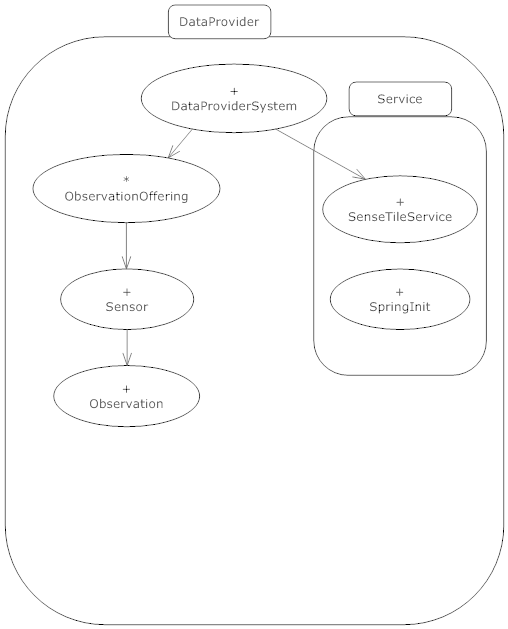
\includegraphics{bon_static_diagam_provider.png}}
\caption{SOS Static Diagram}\label{fig:bon_static_diagam_provider.png}
\end{figure}
The SOS is the main cluster and the Service cluster contains the classes that provide the Web Service interface.

The DataProvider maintains a list of observation offerings provided by the SOS using the ObservationOffering class. When a new sensor type is registered a new ObservationOffering is created. If a DataProvider registers and provides an offering that already exists then just a new Sensor instance is added to the existing ObservationOffering.
 
The Sensor class contains a list of Observations that hold the observations from the DataProvider. The last 50 observations are maintained.

The ObservationService class provides the interface for the DataProducer to update with observations.

The SenseTile Service provides Web Service interface to be used by clients to access the sensor observations.

The SOS specification provides a very rich filtering feature that is too complex for this prototype. The operations are developed in a way to allow the sensor metadata and observations to be retrieved for a specific sensor board. The latest observation or all the stored observations can be retrieved.

\chapter{Implementation}
\section{Overview}
The SenseTile Web Service is written in Java. As described in the high level design there are two components, the DataProducer and the SOS, that are developed to provide this service. The two components are run in separate processes. The communication between the DataProducer and the SOS uses Java RMI. RMI is used due to the SOS and DataProducer
processes are running in the SenseTile Network and communicate over a LAN. This communication protocol has lower overhead than a Web Service so efficient communication between the DataProducer and SOS is achieved. Though it would not be hard to change to use a Web Service as a Java Interface is used to hide the communication mechanism from the main application code. Clients, SOS DataConsumers, access the SOS using a SOAP based Web Service interface. 

The SOS specification describes an implementation using HTTP carry complete operation information encoded in XML including the operations name and parameters. The SenseTile WebService takes a different approach. The operation is defined in the RMI interface and the Web Service Interface while the parameters are encoded in XML thus need parsing.

The following sections describe the DataProducer and SOS implementation.
\section{DataProducer}
The DataProducer, described in section \ref{DataProducerHigh}, accesses the sensor board data and inserts observations into the SOS. Two libraries are used to achieve this: the SensorBoardDriver and the VastSensorMLEngine.

The SensorBoardDriver is described previously in section \ref{SensorBoardDriverSec}. There is also a SensorBoard Simulator library developed by UCS CASL researchers. It produces sensor board packets that can be feed into the DataProvider. This was used during the development of the DataProvider to facilitate testing. 

The VastSensorMLEngine, described in section \ref{VastSensorMLEngineSec}, is used in conjunction with the SenseTile SensorML Model (section \ref{SenseTileModelSec}). The SensorML is parsed by the VastSensorMLEngine into a DOM tree. To perform the processing it propagates an execute method to the instantiated processes. A ProcessMap.xml file maps SensorML ProcessModel and Component method  URNs  (see section \ref{SMLsection}) to Java classes that provide the implementation of the processing to be performed. 

There is no documentation that I can find for the VastSensorMLEngine. There are some reference implementations of SWE services pointed to from the OGC SWE website \footnote{http://www.ogcnetwork.net/SWE} that provide some information how to use it. The SenseTile SensorML model was not parsed initially by the VastSensorMLEngine. As it opensource the code is available and after a few small changes the model parsed. The VastSensorMLEngine processes the model fine and was very stable during testing.


\section{SOS}
The SOS is the provider of the Web Service interface and is built on Apache Axis2 \footnote{http://ws.apache.org/axis2}. 
Axis2 is described as a "Web Services / SOAP / WSDL engine"  with the Apache Axis2/Java implementation used in this thesis. The Spring framework\footnote{http://www.springsource.org/} was also used. Using these libraries a light Web Service is built to run on the reasonably powerful SenseTile Processor Unit. Axis2 is run standalone here though it can be on with any Servlet engine if a more powerful Web Service is needed.

Developing a Web Service is straight forward with Axis2 and it supports several approaches. The supported POJOs (Plain Old Java Objects) approach was used for the SenseTile Web Service as straight forward and the code could be reused on a different framework if AXIS2 did not work well. The Spring framework, which Axis2 supports, was also used for it's dependency injection functionality. A SprinitInit class is needed for Axis to load up the framework.

Axis2 a tool that automatically generates WSDL from the running Web Service. Another tool allows client side code to be generated from the WSDL easing the development of the Web Service clients.

JAXB \footnote{http://java.sun.com/developer/technicalArticles/WebServices/jaxb} was used for SensorML XML to Java binding in the Web Service. JAXB is able to generate a default binding from the complex SWE schema. Some name collisions were corrected with a JAXB customization file found on the SensorML newsgroups.


\chapter{Results}

A  SensorML Model description of a SenseTile Sensor Board and Thermistor was developed. It was
run on a SensorML engine. Appendix shows the model developed.

Developed lighweight Web Service to explore the use of SensorML in Sensor Networks.
running prototype tested with UCD SensorBoard Simulator code.

Tested on a low power Atom PC that is used as SenseTile Processing Unit.

BON mapping developed for main SensorML types. A BON description of SenseTile SensorML Model
was developed based on the mapping.

\chapter{ Conclusions and Future Work}
This thesis analyses the role SensorML plays in Sensor Web Networks. The UCD CASL SenseTile System is used a case study with the development of the SenseTile Web Service to access the SenseTile System sensor data. SensorML alone is not sufficient to model all aspects of Sensor Web Networks but is focused on providing a standard way to exchange sensor metadata, describing sensor input/output data and the processing of sensor data. This leads to examining other OGC SWE specifications, of which SensorML is one. The SWE SOS specification describes the operations for accessing sensor observations and it's concepts were used to develop the SenseTile Web Service. It uses SensorML provide sensor metadata to clients and the O\&M specification to encode observations. The OGC SWE initiative is trying to standardize a Web Service approach to accessing and processing sensor data.

SensorML is relatively intuitive but it is difficult to know if one has developed a "good" SensorML model. There are examples and tutorials to help. 

The SenseTile model uses a hierarachy to model the SenseTile. It seems repetitive to have keep defining the same inputs for each contained component. Maybe this is a flaw in the SenseTile model developed.

Working in XML is error prone. SensorML connections type was a good example of where a graphical tool or another language, like BON,  that can be parsed should be used to check the connections. Running the model through the VastSensorMLEngine without a crash was only way other than by eye to see that the connections were set up correctly. 

SensorML is defined by a heavy XML Schema. This XML Schema along with the other XML Schema for the SOS and dependent specifications are heavy indeed. Achieving a Java binding was difficult. JIBX would not generate a default XML binding. JAXB could with some help. There are many layers of abstraction in these XML Schema. This reflects the that the specifications cover a very wide range of needs of a senor system.

The idea of automatically obtaining a SensoML model and executing it depends on the SensorML Engine being used. Only one Java implementation can be pointed. In the OGC examples the Java implementations of the 

Vast Lib use as a references only.
Had to update library code to get it to work with the SenseTile schema even though the schema
passed the validation test tool from the site. It uses DOM but XML binding is probably a better approach.


the weaknesses of your approach
-----------------------------------------
SOS on the Processor Board. Is this right? RMI only useful if SenseTile Network is a lan.


SWE not fully web services as W3C might define. Not SOAP. HTTP envelope
flexible. There seems to be work ongoing to change this to a more industry standard view of Web Services with the use of WSDL/SOAP. I could not find this as part of current OGC SWE framework.
what has been achieved


further work.
---------------
Complete BON mapping and parser.
Streaming the data. See SWE Architecture dpcument for a description of one approach.
Other technology approaches such as . Other ways such a XQUERY? XML techs?

\newpage
\begin{thebibliography}{99}
\bibitem{OSWAref} Chu, Kobialka,  Durnota, and  Buyya, Open Sensor Web Architecture: Core Services
\bibitem{SMLref}Open Geospatial Consortium Inc., OpenGIS Sensor Model Language (SensorML) Implementation Specification, 2007
\bibitem{SOSref}Open Geospatial Consortium Inc.,  Sensor Observation Service, 2007
\bibitem{OMref}Open Geospatial Consortium Inc., Observations and Measurements – Part 1 - Observation schema, 2007
\bibitem{SWEArchref}Open Geospatial Consortium Inc., OGC Sensor Web Enablement Architecture, 2008
\bibitem{SMLTutorialref}Open Geospatial Consortium Inc., Using SensorML to describe a
Complete Weather Station , 2006
\bibitem{ProcessTutorialref}Open Geospatial Consortium Inc.,
\bibitem{OGCcatref}Open Geospatial Consortium Inc., OpenGIS® Catalogue Services Specification, 2007
\bibitem{BONref}Kim Waldén and Jean-Marc Nerson , "Seamless Object-Oriented Software Architecture", 1995
\end{thebibliography}
\label{endpage}


\chapter{Appendices}
\section{SenseTile SensorML Model}

\lstinputlisting{Thermistor.xml}


\section{BON to SensorML Mapping}
\lstset{basicstyle=\scriptsize,showspaces=false,showstringspaces=false}
\lstinputlisting{SensorML_formal.bon}


\end{document}

\end{article}
